\documentclass{beamer}
\usepackage{amsmath, amssymb}
\usepackage{graphicx}
\usepackage{listings}
\usepackage{color}
\usepackage{subfig}
\usepackage{hyperref}
\usepackage{tcolorbox,fancyvrb,xcolor,tikz}
\tcbuselibrary{skins,breakable}

\usepackage{comment}
% Define a conditional block for skipping
\excludecomment{skipslide}

\newenvironment{VerbatimIN}
 {\VerbatimEnvironment
  \begin{tcolorbox}[
    breakable,
    colback=lightgray,
    spartan
  ]%
  \begin{Verbatim}}
 {\end{Verbatim}\end{tcolorbox}}

 \newenvironment{VerbatimOUT}
 {\VerbatimEnvironment
  \begin{tcolorbox}[
    breakable,
    spartan
  ]%
  \begin{Verbatim}}
 {\end{Verbatim}\end{tcolorbox}}

% R code formatting
\definecolor{codegreen}{rgb}{0,0.6,0}
\definecolor{codegray}{rgb}{0.5,0.5,0.5}
\definecolor{codepurple}{rgb}{0.58,0,0.82}
\definecolor{backcolour}{rgb}{0.95,0.95,0.92}
\lstdefinestyle{Rstyle}{
    backgroundcolor=\color{backcolour},
    commentstyle=\color{codegreen},
    keywordstyle=\color{magenta},
    numberstyle=\tiny\color{codegray},
    stringstyle=\color{codepurple},
    basicstyle=\ttfamily\footnotesize,
    breakatwhitespace=false,
    breaklines=true,
    captionpos=b,
    keepspaces=true,
    numbers=left,
    numbersep=5pt,
    showspaces=false,
    showstringspaces=false,
    showtabs=false,
    tabsize=2
}

\title{Mixed Effects Models - Week 12}
\subtitle{The Bayesian Linear Model II}
\author{Marieke Wesselkamp\\Department of Biometry and Environmental Systems Analysis\\Albert-Ludwigs-University of Freiburg (Germany)}
\date{January 2025}

\begin{document}
\frame{\titlepage}

\begin{frame}
    \frametitle{Recap Last Week}
    Bayesian concepts, explained through Bayes' Theorem:
    \[
    P(\theta|y) = \frac{P(y|\theta) \cdot P(\theta)}{P(y)}
    \]
    with:
    \begin{itemize}
        \item $P(y|\theta)$; The likelihood of the data, given a hypothesis
        \item $P(\theta)$; The prior knowledge, i.e. probability of the hypothesis
        \item $P(\theta|y)$; The posterior probability of the hypothesis, given the data
        \item $P(y)$; The probability of the data
    \end{itemize}
\end{frame}

\begin{frame}
    \frametitle{Recap Last Week}
    \textbf{Sampling from the Posterior}\vspace{0.3cm}
    
     We have one issue in the definition of Bayes' Theorem:
    \[
    P(\theta|y) = \frac{P(y|\theta) \cdot P(\theta)}{P(y)}
    \]
    \vspace{0.2cm}

    \textit{The probability of our hypothesis GIVEN the data is the probability of the data given the hypothesis times the prior knowledge of the observations, standardized by the probability of the data.}
    \vspace{0.2cm}

    \textbf{We avoid the problem by sampling from the posterior distribution} $\mathbf{P(\theta|y)}$
\end{frame}

\begin{frame}
    \frametitle{The Sleepstudy}
    \begin{columns}
        \begin{column}{0.45\textwidth}
            \Large
            Quantifying effects of sleep deprivation on reaction times of participants\\
            \textit{What groupings do we have?}
        \end{column}
        \begin{column}{0.55\textwidth}
            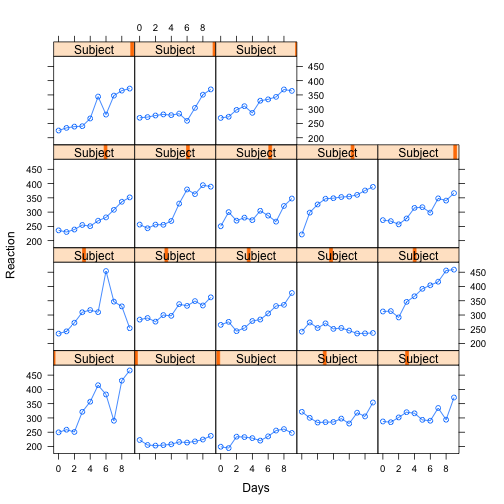
\includegraphics[width=\textwidth]{lectures/day_12_bayesian_lm_II/figures/unnamed-chunk-2-1.png}
        \end{column}
    \end{columns}
\end{frame}

\begin{frame}[fragile]
    \frametitle{Business as usual:}
    We fit a varying intercept and slope model in lme4
    \tiny
    \begin{VerbatimIN}[numbers=left,numbersep=6pt][numbers=left,numbersep=6pt]
mod <- lmer(Reaction ~ Days + (Days|Subject), data=sleepstudy)
summary(mod)
    \end{VerbatimIN}
    \begin{VerbatimOUT}[numbers=left,numbersep=6pt][numbers=left,numbersep=6pt]
Linear mixed model fit by REML ['lmerMod']
Formula: Reaction ~ Days + (Days | Subject)
   Data: sleepstudy

REML criterion at convergence: 1743.6
Scaled residuals: 
    Min      1Q  Median      3Q     Max 
-3.9536 -0.4634  0.0231  0.4634  5.1793 
Random effects:
 Groups   Name        Variance Std.Dev. Corr
 Subject  (Intercept) 612.10   24.741       
          Days         35.07    5.922   0.07
 Residual             654.94   25.592       
Number of obs: 180, groups:  Subject, 18
Fixed effects:
            Estimate Std. Error t value
(Intercept)  251.405      6.825  36.838
Days          10.467      1.546   6.771

Correlation of Fixed Effects:
     (Intr)
Days -0.138
    \end{VerbatimOUT}
\end{frame}

\begin{frame}
    \frametitle{}
    \centering
    \huge\color{purple}\textbf{What do we need to fit this model in the Bayesian way?}
\end{frame}

\begin{frame}
    \frametitle{}
    So far, we used the following notation to formalize a regression model:
    \[
    \mathbf{y} = \beta_0 + \beta_1 \cdot \mathbf{X} + \epsilon
    \]
    with:
    \[
    \epsilon_{iid} \sim Normal(0, \sigma_{\epsilon}^2)
    \]
    \vspace{0.2cm}
    
    Since last week we know, that this notation is equivalent to:
    \[
    \mathbf{y} \sim Normal(\mu, \sigma_{\epsilon}^2)
    \]
    with:
    \[
    \mu = \beta_0 + \beta_1 \cdot \mathbf{X}
    \]
\end{frame}

\begin{frame}
    \frametitle{New Notation for the Varying Intercept Model}
    \large
    \begin{align*}
        &\mathbf{Reaction} \sim Normal(\mu, \sigma_{e}) \\
        &\mu = \alpha + \alpha_{SUBJECT[i]} + \beta \cdot \mathbf{Days} \quad \text{for i in 1, ...subjects}\\
        &\alpha_{SUBJECT} \sim Normal(0, \sigma_{SUBJECT}) \\
        &\alpha \sim Normal(0, 10) \\
        &\beta \sim Normal(0, 10) \\
        &\sigma_{e} \sim HalfCauchy(0,1) \\
        &\sigma_{SUBJECT} \sim HalfCauchy(0,1)
    \end{align*}

    \vspace{1cm}
    How does the Half-Cauchy distribution look like? Check it out at the \href{https://distribution-explorer.github.io/continuous/halfcauchy.html}{Distribution explorer}.
\end{frame}

\begin{frame}
    \frametitle{New Notation for the Varying Intercept Model}
    \large
    \begin{align*}
        & \mathbf{Reaction} \sim Normal(\mu, \sigma_{e}) \quad \text{Likelihood}\\
        & \mu = \alpha + \alpha_{SUBJECT[i]} + \beta \cdot \mathbf{Days} \quad \text{Linear Model}\\
        & \alpha_{SUBJECT} \sim Normal(0, \sigma_{SUBJECT}) \quad \text{Prior for varying intercept}\\
        & \alpha \sim Normal(0, 10) \quad \text{Prior for population intercept}\\
        & \beta \sim Normal(0, 10) \quad \text{Prior for population slope}\\
        & \sigma_{e} \sim HalfCauchy(0,1) \quad \text{Prior for stddev within subjects}\\
        & \sigma_{SUBJECT} \sim HalfCauchy(0,1) \quad \text{Prior for stddev among k subjects}
    \end{align*}
\end{frame}

\begin{skipslide}
\begin{frame}[fragile]
    \frametitle{The Sleepstudy in JAGs}
    \tiny
    \begin{VerbatimIN}[numbers=left,numbersep=6pt]
jagsmodel <- textConnection('
                            model {
                            # prior
                            for (j in 1:k){
                              alpha ~ dnorm(alpha0, tau.ranI)
                            }
                            alpha0 ~ dnorm(300, 0.001)
                            tau.ranI ~ dgamma(0.001, 0.001)

                            beta ~ dnorm(0, 10)
                            tau ~ dgamma(0.001, 0.001)

                            sigma.ranI <- 1/sqrt(tau.ranI)
                            sigma <- 1/sqrt(tau)

                            # likelihood
                            for (i in 1:N){
                              # model
                              mu[i] <- alpha0 + alpha[Subject[i]] + beta*Days[i]
                              Reaction[i] ~ dnorm(mu[i], tau) 
                              # mean and precision (=1/variance)
                            }
                            }
                            ')
parameters <- c("alpha", "alpha0", "beta", "sigma", "sigma.ranI")
    \end{VerbatimIN}
    \normalsize
    How would you specify the random intercept random slope model?
\end{frame}
\end{skipslide}

\begin{frame}[fragile]
    \frametitle{The Sleepstudy in brms}
    In brms (\textit{Bayesian Linear Regression Models using Stan}) we can specify this model in the lme4 syntax:
    \scriptsize
    \begin{VerbatimIN}[numbers=left,numbersep=6pt]
bmod <- brm(Reaction ~ Days + (Days|Subject), data = sleepstudy, 
            family = gaussian())
    \end{VerbatimIN}
    \vspace{0.2cm}
    
    \normalsize
    brms internally creates code in Stan, which can be accessed:
    \scriptsize
    \begin{VerbatimIN}[numbers=left,numbersep=6pt]
stancode(bmod)
    \end{VerbatimIN}
\end{frame}

\begin{frame}[fragile]
    \frametitle{The Random Intercept Model in Stan}
    \tiny
    \begin{VerbatimIN}[numbers=left,numbersep=6pt]
data {
    int N;
    real Reaction[N];
    real Days[N];
    int subject_index[N];
    int N_subject_index;
}
parameters {
    real Intercept;
    real beta_Days;
    real<lower=0> sigma;
    real<lower=0> sigma.ranI;
    real vary_subject_index[N_subject_index];
}
model {
    real vary[N];
    real glm[N];
    // Priors
    Intercept ~ normal( 0 , 100 );
    beta_Days ~ normal( 0 , 100 );
    sigma ~ uniform( 0 , 100 );
    sigma.ranI ~ uniform( 0 , 100 );
    // Varying effects;
    for ( j in 1:N_subject_index ) vary_subject_index[j] ~ normal( zeros_subject_index 
    , sigma.ranI );
    // Fixed effects
    for ( i in 1:N ) {
        vary[i] <- vary_subject_index[subject_index[i],1];
        glm[i] <- vary[i] + Intercept + beta_Days * Days[i];
    }
    Reaction ~ normal( glm , sigma );
}
    \end{VerbatimIN}
\end{frame}

\begin{frame}[fragile]
    \frametitle{Setting Priors for your brms model}
    We can access an overview of priors that can be specified, as well as their defaults:
    \tiny
    \begin{VerbatimIN}[numbers=left,numbersep=6pt]
get_prior(Reaction ~ Days + (Days|Subject), data=sleepstudy)
    \end{VerbatimIN}
    \begin{VerbatimOUT}[numbers=left,numbersep=6pt]
                     prior     class      coef   group resp dpar nlpar lb ub       source
                    (flat)         b                                              default
                    (flat)         b      Days                               (vectorized)
                    lkj(1)       cor                                              default
                    lkj(1)       cor           Subject                       (vectorized)
 student_t(3, 288.7, 59.3) Intercept                                              default
     student_t(3, 0, 59.3)        sd                                    0         default
     student_t(3, 0, 59.3)        sd           Subject                  0    (vectorized)
     student_t(3, 0, 59.3)        sd      Days Subject                  0    (vectorized)
     student_t(3, 0, 59.3)        sd Intercept Subject                  0    (vectorized)
     student_t(3, 0, 59.3)     sigma                                    0         default
    \end{VerbatimOUT}
    \normalsize
    Further information is well documented and accessible through ?prior
\end{frame}

\begin{frame}[fragile]
    \frametitle{Setting Priors for your brms model}
    Change the flat priors for our $\beta$ to informative priors. So we set them to normal, using the \textit{b-class}. For the random variance components we set a HalfCauchy or Gamma prior, using the \textit{sd-class}: \vspace{0.2cm}
    
    \scriptsize
    \begin{VerbatimIN}[numbers=left,numbersep=6pt]
prior <- c(
    prior(normal(0, 10), class = b),
    prior(cauchy(0, 1), class = sd)
    )
    \end{VerbatimIN}
\end{frame}

\begin{frame}[fragile]
    \frametitle{Let's fit the model:}
    \begin{itemize}
        \item specify family
        \item specify your priors
        \item choose warm-up steps, full iteration steps and the number of chains
    \end{itemize}
    \scriptsize
    \begin{VerbatimIN}[numbers=left,numbersep=6pt]
bmod <- brm(
    Reaction ~ Days + (Days|Subject),
    data = sleepstudy, family = gaussian(),
    prior = prior,
    warmup = 1000, iter = 5000, chain=4,
    save_pars = save_pars(all=TRUE) # for marginal likelihood
    )
    \end{VerbatimIN}
    \normalsize
    Compiling to Stan and the sampling procedure will take some time
\end{frame}

\begin{frame}[fragile]
    \frametitle{Adjusted Prior Assumptions}
    Print the adjusted Prior assumptions of the model:
    \tiny
    \begin{VerbatimIN}[numbers=left,numbersep=6pt]
prior_summary(bmod)
    \end{VerbatimIN}
    \begin{VerbatimOUT}[numbers=left,numbersep=6pt]
                     prior     class      coef   group resp dpar nlpar lb ub       source
             normal(0, 10)         b                                                 user
             normal(0, 10)         b      Days                               (vectorized)
 student_t(3, 288.7, 59.3) Intercept                                              default
      lkj_corr_cholesky(1)         L                                              default
      lkj_corr_cholesky(1)         L           Subject                       (vectorized)
              cauchy(0, 1)        sd                                    0            user
              cauchy(0, 1)        sd           Subject                  0    (vectorized)
              cauchy(0, 1)        sd      Days Subject                  0    (vectorized)
              cauchy(0, 1)        sd Intercept Subject                  0    (vectorized)
     student_t(3, 0, 59.3)     sigma                                    0         default
    \end{VerbatimOUT}
\end{frame}

\begin{frame}[fragile]
    \frametitle{Model Summary}
    Check the model fit for Convergence Issues and Sampling Efficiency. We can use the model summary in lme4:
    \tiny
    \begin{VerbatimOUT}[numbers=left,numbersep=6pt]
Linear mixed model fit by REML ['lmerMod']
Formula: Reaction ~ Days + (1 | Subject)
   Data: sleepstudy

REML criterion at convergence: 1786.5

Scaled residuals: 
    Min      1Q  Median      3Q     Max 
-3.2257 -0.5529  0.0109  0.5188  4.2506 

Random effects:
 Groups   Name        Variance Std.Dev.
 Subject  (Intercept) 1378.2   37.12   
 Residual              960.5   30.99   
Number of obs: 180, groups:  Subject, 18

Fixed effects:
            Estimate Std. Error t value
(Intercept) 251.4051     9.7467   25.79
Days         10.4673     0.8042   13.02

Correlation of Fixed Effects:
     (Intr)
Days -0.371
    \end{VerbatimOUT}
\end{frame}

\begin{frame}[fragile]
    \frametitle{Model Summary}
    The model summary in brms:
    \tiny
    \begin{VerbatimOUT}[numbers=left,numbersep=6pt]
 Family: gaussian 
  Links: mu = identity; sigma = identity 
Formula: Reaction ~ Days + (Days | Subject) 
   Data: sleepstudy (Number of observations: 180) 
  Draws: 4 chains, each with iter = 5000; warmup = 1000; thin = 1;
         total post-warmup draws = 16000

Group-Level Effects: 
~Subject (Number of levels: 18) 
                    Estimate Est.Error l-95% CI u-95% CI Rhat Bulk_ESS Tail_ESS
sd(Intercept)          23.60      6.36    12.53    37.67 1.00     6603     8357
sd(Days)                5.91      1.31     3.76     8.86 1.00     6402     9552
cor(Intercept,Days)     0.16      0.30    -0.40     0.75 1.00     4184     6049

Population-Level Effects: 
          Estimate Est.Error l-95% CI u-95% CI Rhat Bulk_ESS Tail_ESS
Intercept   251.47      6.76   238.03   264.72 1.00     8449    10322
Days         10.15      1.55     7.07    13.19 1.00     6483     8904

Family Specific Parameters: 
      Estimate Est.Error l-95% CI u-95% CI Rhat Bulk_ESS Tail_ESS
sigma    26.09      1.59    23.24    29.45 1.00    11621    11335

Draws were sampled using sampling(NUTS). For each parameter, Bulk_ESS
and Tail_ESS are effective sample size measures, and Rhat is the potential
scale reduction factor on split chains (at convergence, Rhat = 1).
    \end{VerbatimOUT}
\end{frame}

\begin{frame}
    \frametitle{lme4 vs. brms}
    \begin{itemize}
        \item lme4 returns the variance $\sigma^2$ for group-level effects, instead of the standard deviation $\sigma$
        \item brms returns the 95\% credible intervals for the parameter estimates
        \item In brms, $\hat{R}$ gives information about model convergence
        \item Bulk-ESS and Tail-ESS give information on sampling efficiency and reliability of credible intervals
    \end{itemize}
    \vspace{0.2cm}

    Rules of Thumb:
    \begin{itemize}
        \item $\hat{R}$ should not be much larger than 1.05
        \item Bulk-ESS and Tail-ESS should be at least 100
    \end{itemize}
\end{frame}

\begin{frame}[fragile]
    \frametitle{Graphical Posterior Predictive Checks}
     \begin{columns}
        \begin{column}{0.5\textwidth}
            Sample from the posterior predictive distribution. The density of observed and predicted response. \vspace{0.2cm}
            
            \scriptsize
            \begin{VerbatimIN}[numbers=left,numbersep=6pt]
pp_check(bmod, ndraws=100)
            \end{VerbatimIN}
        \end{column}
        \begin{column}{0.5\textwidth}
            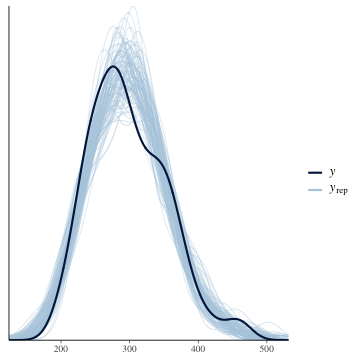
\includegraphics[width=\textwidth]{lectures/day_12_bayesian_lm_II/figures/unnamed-chunk-15-1.png}
        \end{column}
    \end{columns}
\end{frame}

\begin{frame}[fragile]
    \frametitle{Graphical Posterior Predictive Checks}
    Normality of Residuals:
     \begin{columns}
        \begin{column}{0.5\textwidth}
        \scriptsize
            \begin{VerbatimIN}[numbers=left,numbersep=6pt]
pp_check(bmod,type="error_hist",
         ndraws=1)
            \end{VerbatimIN}
            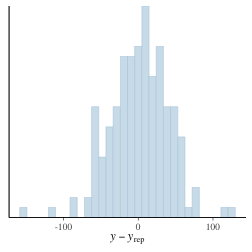
\includegraphics[width=\textwidth]{lectures/day_12_bayesian_lm_II/figures/unnamed-chunk-16-1.png}
        \end{column}
        \begin{column}{0.5\textwidth}
            \scriptsize
            \begin{VerbatimIN}[numbers=left,numbersep=6pt]
pp_check(bmod, type="loo_pit")
            \end{VerbatimIN}
            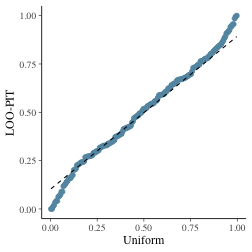
\includegraphics[width=\textwidth]{lectures/day_12_bayesian_lm_II/figures/unnamed-chunk-16-2.png}	
        \end{column}
    \end{columns}
\end{frame}

\begin{frame}[fragile]
    \frametitle{Graphical Posterior Predictive Checks}
    Plot custom posterior distributions of parameters:
    \scriptsize
    \begin{VerbatimIN}[numbers=left,numbersep=6pt]
post_params <- posterior_samples(bmod) # ignore warning
    \end{VerbatimIN}
    \begin{center}
        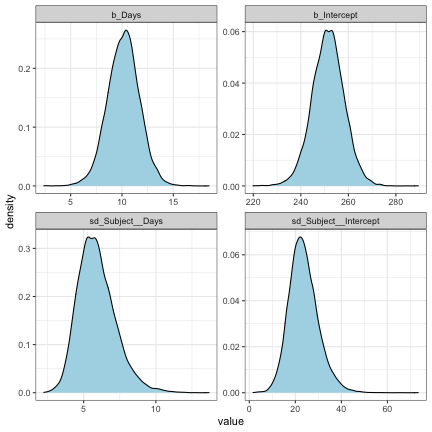
\includegraphics[width=0.5\textwidth]{lectures/day_12_bayesian_lm_II/figures/unnamed-chunk-18-1.png}
    \end{center}
\end{frame}

\begin{frame}[fragile]
    \frametitle{Graphical Posterior Predictive Checks}
    \begin{center}
    How did prior assumptions change? \vspace{0.2cm}
    
        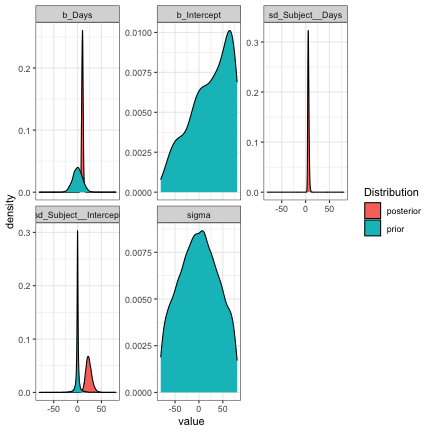
\includegraphics[width=0.6\textwidth]{lectures/day_12_bayesian_lm_II/figures/unnamed-chunk-20-1.png}
    \end{center}
\end{frame}

\begin{frame}[fragile]
    \frametitle{Graphical Posterior Predictive Checks}
     \begin{columns}
        \begin{column}{0.5\textwidth}
            Posterior distributions of varying intercepts:
            \vspace{1.1cm}
            
            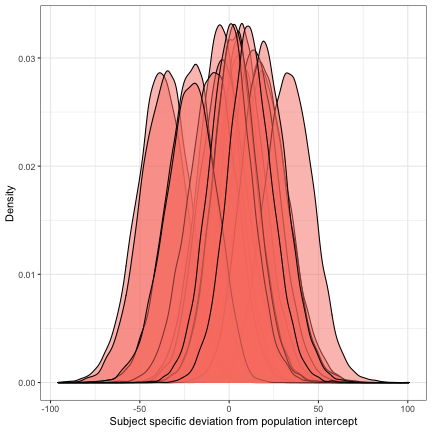
\includegraphics[width=\textwidth]{lectures/day_12_bayesian_lm_II/figures/unnamed-chunk-21-1.png}
        \end{column}
        \begin{column}{0.5\textwidth}
            In contrast: Point estimates and CIs for non-bayesian ranefs:
            \scriptsize
            \begin{VerbatimIN}[numbers=left,numbersep=6pt]
qqmath(ranef(mod))
            \end{VerbatimIN}
            \begin{center}
            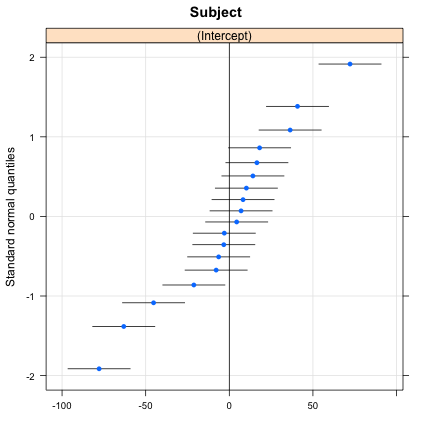
\includegraphics[width=\textwidth]{lectures/day_12_bayesian_lm_II/figures/unnamed-chunk-22-1.png}
            \end{center}
        \end{column}
    \end{columns}
\end{frame}

\begin{frame}[fragile]
    \frametitle{Graphical Posterior Predictive Checks}
    Or plot the posterior distributions and trace plots with the brms default plot:
    \scriptsize
    \begin{VerbatimIN}[numbers=left,numbersep=6pt]
plot(bmod)
    \end{VerbatimIN}
    \begin{columns}
        \begin{column}{0.5\textwidth}
            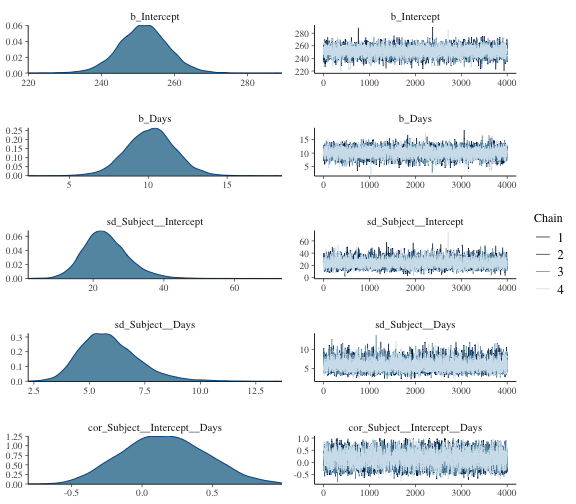
\includegraphics[width=\textwidth]{lectures/day_12_bayesian_lm_II/figures/unnamed-chunk-23-1.png}
        \end{column}
        \begin{column}{0.5\textwidth}
            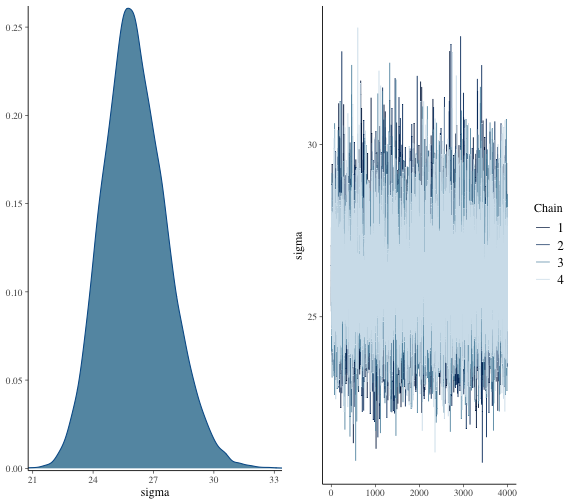
\includegraphics[width=\textwidth]{lectures/day_12_bayesian_lm_II/figures/unnamed-chunk-23-2.png}
        \end{column}
    \end{columns}
\end{frame}

\begin{frame}[fragile]
    \frametitle{Graphical Posterior Predictive Checks}
    Population level predictions with confidence intervals:
    \begin{center}
        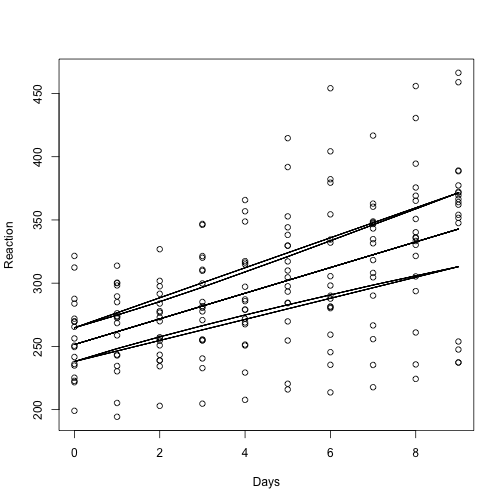
\includegraphics[width=0.45\textwidth]{lectures/day_12_bayesian_lm_II/figures/unnamed-chunk-25-1.png}
    \end{center}
    \tiny
    \begin{VerbatimIN}[numbers=left,numbersep=6pt]
newdata <- data.frame(Days = sleepstudy$Days, Subject = sleepstudy$Subject)
fit <- as.data.frame(fitted(bmod,
              newdata = newdata,
              re_formula = NA, #ignore random effects
              summary = TRUE #summarize posterior(get 95% CI & mean instead of MCMC chain)
              ) )
    \end{VerbatimIN}
\end{frame}

\begin{frame}[fragile]
    \frametitle{Graphical Posterior Predictive Checks}
    Or use the default plots for the population effects:
    \begin{center}
        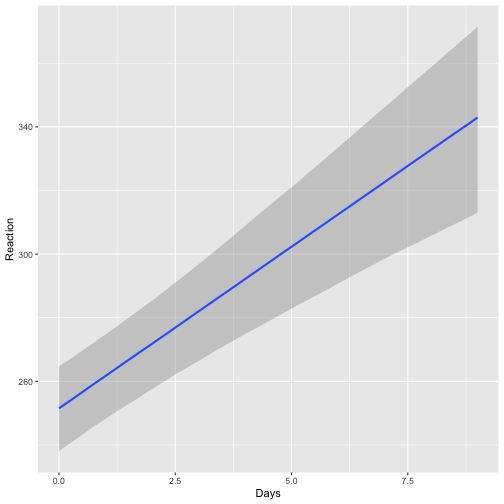
\includegraphics[width=0.5\textwidth]{lectures/day_12_bayesian_lm_II/figures/unnamed-chunk-26-1.png}
    \end{center}
    \scriptsize
    \begin{VerbatimIN}[numbers=left,numbersep=6pt]
conditional_effects(bmod)
    \end{VerbatimIN}
\end{frame}

\begin{frame}[fragile]
    \frametitle{Graphical Posterior Predictive Checks}
    Random effect level predictions (without confidence intervals):
    \begin{center}
        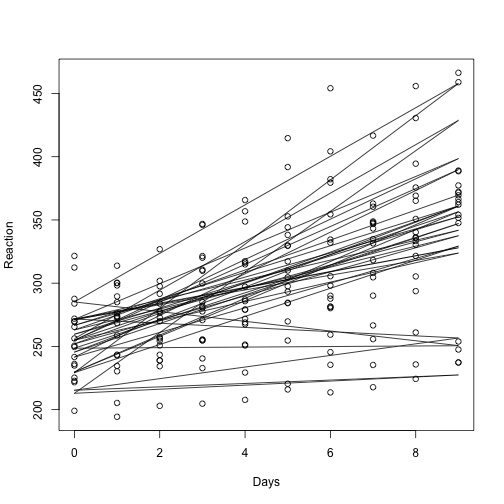
\includegraphics[width=0.45\textwidth]{lectures/day_12_bayesian_lm_II/figures/unnamed-chunk-28-1.png}
    \end{center}
    \tiny
    \begin{VerbatimIN}[numbers=left,numbersep=6pt]
newdata <- data.frame(Days = sleepstudy$Days, Subject = sleepstudy$Subject)
fit <- as.data.frame(fitted(bmod,
              newdata = newdata,
              re_formula = NULL, #include random effects
              summary = TRUE #summarize posterior (get 95% CI & mean instead of MCMC chain)
              ) )
    \end{VerbatimIN}
\end{frame}

\begin{frame}
    \frametitle{Model Diagnosis: summary}
    \large
    \textbf{brms specific:}
    \begin{itemize}
        \item Check $\hat{R}$
        \item Check Bulk\textunderscore ESS and Tail\textunderscore ESS 
        \item Trace plots and posterior distributions
    \end{itemize}
    \vspace{0.2cm}

    \textbf{Other checks:}
    \begin{itemize}
        \item Variance components
        \item Residuals
    \end{itemize}
\end{frame}

\begin{frame}
    \frametitle{Model Selection Criterion}
    \large
    In non-bayesian models we use the AIC or BIC to approximate the predictive accuracy. The AIC estimates the average out-of-sample deviance as:
    \[
    AIC = -2ln(L) + 2p
    \]
    Where $D_{train}$ is the in sample deviance and $p$ the number of free parameters to be estimated. \vspace{0.2cm}

    \textbf{BUT:} It assumes flat priors, an approximately multivariate gaussian posterior and a sample size much greater than $p$
\end{frame}

\begin{frame}
    \frametitle{The Widely Applicable Information Criterion (WAIC)}
    \large
    Allows for non-gaussian priors and posterior. A \textit{pointwise} information criterion that consists of two parts:\\
    The log-pointwise-predictive-density:
    \[
    lppd = \sum_{i=1}^N log(P(y_i|\theta))
    \]
    The effective number of parameters:
    \[
    p_{WAIC} = \sum_{i=1}^N Var[log(P(y_i|\theta))]
    \]
    Together they give the WAIC:
    \[
    WAIC = -2(lppd - p_{WAIC})
    \]
\end{frame}

\begin{frame}[fragile]
    \frametitle{Application of WAIC}
    \scriptsize
    \begin{VerbatimIN}[numbers=left,numbersep=6pt]
bmod2 <- brm(Reaction ~ Days + (1|Subject),
    data = sleepstudy, family = gaussian(),
    prior = prior,
    warmup = 1000, iter = 5000, chain=4,
    save_pars = save_pars(all=TRUE))
bmod <- add_criterion(bmod, "waic")
bmod2 <- add_criterion(bmod2, "waic")

loo_compare(bmod2, bmod, criterion="waic")
    \end{VerbatimIN}
    \begin{VerbatimOUT}[numbers=left,numbersep=6pt]
      elpd_diff se_diff
bmod    0.0       0.0  
bmod2 -24.0      11.1  
    \end{VerbatimOUT}
\end{frame}

\begin{frame}[fragile]
\frametitle{Application of WAIC}
    \begin{columns}
        \begin{column}{0.5\textwidth}
            \scriptsize
            \begin{VerbatimIN}[numbers=left,numbersep=6pt]
bmod$criteria$waic
            \end{VerbatimIN}
            \begin{VerbatimOUT}[numbers=left,numbersep=6pt]
Computed from 16000 by 180 
log-likelihood matrix

          Estimate   SE
elpd_waic   -860.6 21.8
p_waic        32.0  8.0
waic        1721.2 43.6

13 (7.2%) p_waic estimates 
greater than 0.4. We recommend 
trying loo instead. 
            \end{VerbatimOUT}
        \end{column}
        \begin{column}{0.5\textwidth}
            \scriptsize
            \begin{VerbatimIN}[numbers=left,numbersep=6pt]
bmod2$criteria$waic
            \end{VerbatimIN}
            \begin{VerbatimOUT}[numbers=left,numbersep=6pt]
Computed from 16000 by 
180 log-likelihood matrix

          Estimate   SE
elpd_waic   -884.6 14.3
p_waic        19.0  3.3
waic        1769.2 28.6

9 (5.0%) p_waic estimates 
greater than 0.4. We recommend 
trying loo instead. 
            \end{VerbatimOUT}
        \end{column}
    \end{columns}
\end{frame}

\begin{frame}[fragile]
    \frametitle{Hypothesis Testing}
    \large
    lmerTest does not work for brms models. Instead we use \textbf{Bayes Factor}, the Bayesian likelihood ratio. We require enough posterior samples to calculate this.
    \scriptsize
    \begin{VerbatimIN}[numbers=left,numbersep=6pt]
bf1 <- bayes_factor(bmod, bmod2, log=TRUE)
    \end{VerbatimIN}
    \begin{VerbatimOUT}[numbers=left,numbersep=6pt]
Estimated log Bayes factor in favor of bmod over bmod2: 14.41752
    \end{VerbatimOUT}
    \large
    A small Bayes factor (close to 0) refers to small differences in hypothesis. No NSHT framework, no p-values!
\end{frame}

\begin{frame}
    \frametitle{Hypothesis Testing}
    \large
    \begin{columns}
        \begin{column}{0.5\textwidth}
            Bayes factor for two models with equal prior probability approaches the posterior probability ratio ($\alpha$)
            \[
            K = \frac{P(\theta_1|Y)P(\theta_1)}{P(\theta_2|Y)P(\theta_2)}
            \]
        \end{column}
        \begin{column}{0.5\textwidth}
            Scale interpretation:
            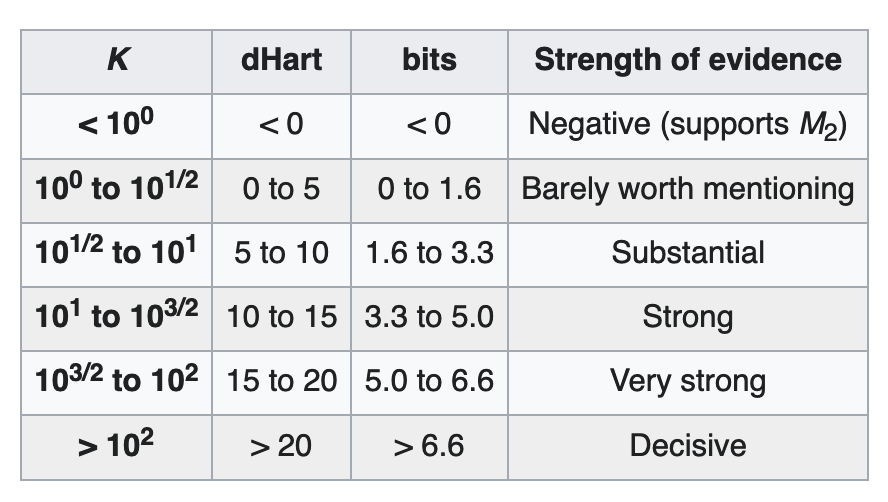
\includegraphics[width=\textwidth]{lectures/day_12_bayesian_lm_II/figures/bayesfactor.png}
        \end{column}
    \end{columns}
\end{frame}

\begin{frame}[fragile]
    \frametitle{What is this all about?}
    Remember the bloodworms data:
    \scriptsize
    \begin{VerbatimIN}[numbers=left,numbersep=6pt]
mod.prop.1 <- glmer(prop ~ Temp * poly(Food,3) 
                    + Length + Trial_Split 
                    + (Trial_Split|Week_Block/ID), 
                    family = binomial, data = ing, weights = Food,
                    control = glmerControl(optimizer = "nlminbwrap", 
                                           check.conv.grad  = 
                                           .makeCC("warning", 
                                           tol=1e-2, relTol=NULL)))
    \end{VerbatimIN}
    \normalsize
    Advantages of modeling the bloodworms data in brms:
    \begin{itemize}
        \item allows modeling of zero-inflated or over-dispersed data
        \item allows modeling of data with non-gaussian errors and random variances
        \item a more robust estimation procedure, as such less convergence issues
    \end{itemize}
\end{frame}

\begin{frame}
    \frametitle{Recapitulation Week 12}
    Concepts of today:
    \begin{itemize}
        \item New notation for regression models
        \item Fitting a Bayesian mixed effects models in brms
        \item New information criterion for BMEMs
        \item Hypothesis tests for BEMs
    \end{itemize}
    \vspace{0.3cm}
    
    Todays Exercises:\\
    Practice Bayesian model fitting with brms
\end{frame}
\end{document}